\chapter{Implementación}

\section{Estimación de costes}

Estimamos el coste a partir
del desglose del capítulo anterior y de datos pasados que
tenemos en otros proyectos, tal y como se explica en el
segundo capítulo.

\begin{table}[!h]
    \centering
    \begin{tabular}{|l|c|c|c|}
    \hline
    \multicolumn{1}{|c|}{\textbf{Nombre}}                                                                                               & \textbf{Horas estimadas}   & \textbf{Días estimados} & \begin{tabular}[c]{@{}c@{}}\textbf{Número de registros}\\ \textbf{en los que se basa}\\ \textbf{esta afirmación}\end{tabular} \\ \hline \hline
    \begin{tabular}[c]{@{}l@{}}Modelado de las reglas de\\ procesamiento de eventos\\ (registro)\end{tabular}                  & 8$\sim$11,5 horas & 2$\sim$3 días  & 3                                                                                                  \\ \hline
    \begin{tabular}[c]{@{}l@{}}Modelado de las reglas de\\ almacenamiento y recuperación\\ de eventos (registros)\end{tabular} & 8$\sim$15,5 horas & 2$\sim$3 días  & 3                                                                                                  \\ \hline
    Driver FRAM                                                                                                                & 3$\sim$6 horas    & 1$\sim$2 días  & 2                                                                                                  \\ \hline
    Integración con HMI                                                                                                        & 1$\sim$9 horas    & 1$\sim$2 días  & 15                                                                                                 \\ \hline
    \end{tabular}
\end{table}

Estimamos que el trabajo puede llevar 10 días de trabajo.

El coste de oportunidad de estos 10 días dependerá de los
proyectos que podamos tener sobre la mesa y de sus circunstancias.
Tendremos que tener en cuenta también el coste en tiempo
para el soporte que daremos en el prototipo.

Para coste monetario (únicamente gastos) tenemos que tener en cuenta
entre otros:

\begin{enumerate}[noitemsep,nolistsep]
    \item \textbf{Coste de la empresa}. Es decir, cuánto me
          cuesta al día tener la empresa funcionando.
          En nuestro caso tenemos en cuenta los gastos
          derivados por:
        \begin{itemize}[noitemsep,nolistsep]
            \item Gestión fiscal.
            \item Lugar de trabajo (oficina).
            \item Almacén.
            \item Transporte.
            \item Equipamiento de laboratorio. (Coste amortizado)
            \item Estaciones de desarrollo. (Coste amortizado)
            \item Líneas de teléfono e Internet.
            \item Licencias Software.
        \end{itemize}
    \item \textbf{Coste de los servicios} que ofrezco yo y mi
          colaborador. Las facturas que emitimos.
    \item \textbf{Coste de los viajes para celebrar las reuniones}.
    \item \textbf{Coste de los viajes para probar los prototipos}.
    \item \textbf{Coste de soporte y formación}. Más difícil de cuantificar
          en tanto que ocurrirá en el futuro y no sabemos
          cuánto tiempo ocupará.
\end{enumerate}

\begin{figure}[h]
    \centering
    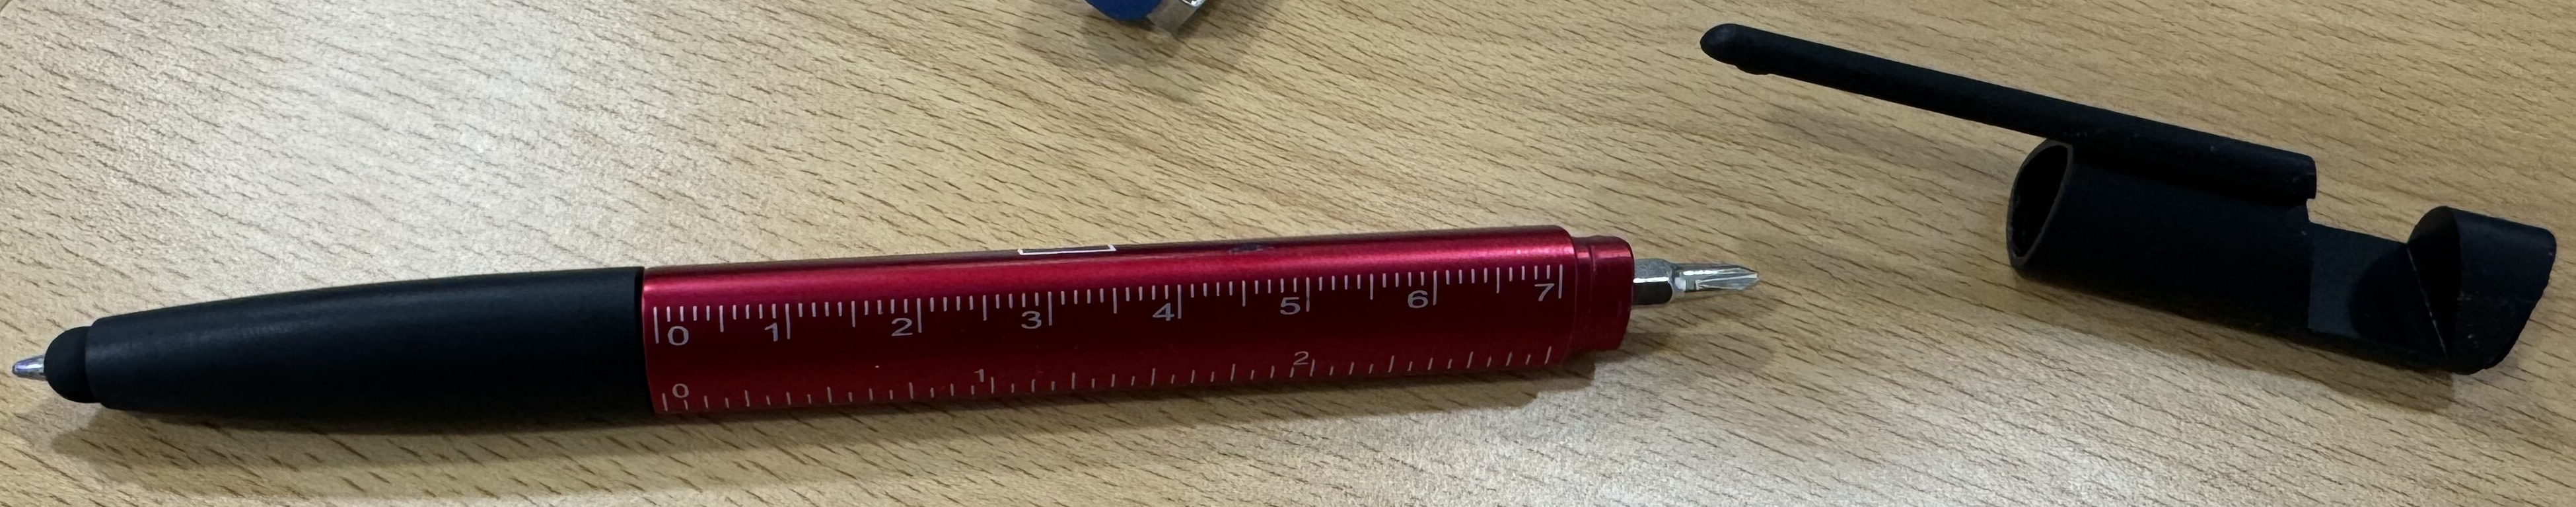
\includegraphics[width=\textwidth]{boligrafo-wurt.jpg}
    \caption{La gestión de un almacén es una tarea recurrente, tediosa y cara. Sin embargo,
    gracias a estar en contacto con vendedores, podemos disfrutar del bolígrafo de
    Würth Elektronik, que
    no sólo nos permite escribir, sino que además nos sirve de regla, destornillador,
    apuntador táctil, sujeta-móviles y hasta nos permite borrar una pizarra blanca.}
\end{figure}

\section{Entorno de desarrollo}

El diseño e implementación del entorno de desarrollo lo
vamos desarrollando a medida que vamos necesitándolo.
A lo largo del desarrollo del proyecto declaramos las
siguientes historias de desarrollador.

\subsection{HD1: Correctitud del contenido del repositorio}

\textit{Como desarrollador, quiero asegurarme que en ningún
momento hago un push de commits que no superan
la comprobación de calidad, de forma que no puedan
romper la entrega continua. Quiero poder ver en Github
que la ejecución de los scripts de comprobación se han
ejecutado correctamente y que no han encontrado errores.}

\subsubsection{Solución implementada}

Nuestra empresa utiliza Github. Github permite ejecutar
scripts sobre contenedores tanto en sus servidores como
en local.

Por cada script de comprobación a ejecutar declaramos
un flujo de trabajo de Github. En la página web del
repositorio vemos junto a los commits correspondientes
el resultado de la ejecución de los flujos de trabajo
en los servidores de Github.
Los flujos de trabajo los encontramos bajo el directorio
\texttt{.github}.

Para asegurar el correcto estado del repositorio en cada
contribución ejecutamos \texttt{act}, una herramienta
desarrollada por Github disponible en Linux, MacOS y Windows,
la cual se encarga de lanzar los flujos de trabajo
a través de contenedores \textit{Docker}. En caso de
no superar algún flujo de trabajo no permitimos añadir
la contribución al repositorio.

La automatización de la ejecución de \texttt{act} en cada
intento de contribución la conseguimos mediante la funcionalidad
de \texttt{git} \textit{Git Hooks}. El desarrollador tiene
que activar esta funcionalidad ejecutando el script \texttt{dev-setup.sh}

\subsection{HD2: Integración con \textit{SDK} de Renesas}

\textit{Como desarrollador quiero que el software que desarrolle
se pueda importar fácilmente en un proyecto que utilice
la plataforma de desarrollo \textit{e2studio}, de forma que pueda
importar trozos de código desde un proyecto \textit{RA FSP}
sin tener que modificar las fuentes originales. De esta forma puedo
tener submódulos de git que sean parte del proyecto principal.
Utilizamos la familia de microprocesadores RA6M1.}

\subsubsection{Solución implementada}

En la raíz de los directorios de las librerías que implementamos
incluimos los ficheros que necesita \texttt{e2studio} para
saber cómo compilar el código. Declaramos que debe compilar
pensando en que la plataforma objetivo es del tipo Cortex-M4.
Declaramos que las instrucciones en coma flotante deben ejecutarse
sobre la FPU utilizando la especificación ABI \texttt{fpv4-sp-d16}.

\subsection{HD3: Comprobación automática del correcto comportamiento del software}

\textit{Como desarrollador quiero practicar TDD porque es mi mejor
método para desarrollar código correcto. Únicamente necesitaré
aserciones básicas, aunque es muy importante que pueda depurar
de una forma rápida y sencilla dado un trozo de código
que no entienda por qué no funciona. Como trabajo con más gente,
y esta gente no tiene por qué tener mis herramientas de desarrollo
ni pararse a preparar una plataforma de desarrollo, necesito que
cualquiera pueda empezar a desarrollar código sin tener que preocuparse
por configurar nada.}

\subsubsection{Solución implementada}

Para el caso del desarrollo del driver de la memoria, como los tests
deberían poder ejecutarse fácilmente en cualquier plataforma objetivo,
dependemos en el encabezado \texttt{assert.h}. Como es parte de la
especificación ISO C muy probablemente la plataforma objetivo
la implemente como parte de \texttt{libc}. Añadimos el fichero
\texttt{example\_MFHMI.c} como ejemplo de cómo se ejecutan los tests
en una MFHMI.

Para el caso del módulo del histórico de registros utilizamos
Ceedling, ya que no queremos ni que la ejecución de los tests
se ejecute sobre un hardware concreto al no ser necesario y
porque nos proporciona herramientas para compilar unitariamente
el proyecto fácilmente. Ha demostrado ser eficaz y suficiente
en proyectos de este tipo en el pasado, y es una tecnología ya
conocida en la empresa.

Creo imágenes \textit{Docker} de desarrollo que se pueden utilizar en
\textit{Visual Studio Code} para que cualquier persona pueda, sin
necesidad de instalación, contribuir o mantener el repositorio.

\subsection{HD4: Gestión de documentación}

\textit{Como desarrollador quiero poder, dada una versión de programa,
ver la documentación de entonces y poder exportarla a PDF para
poder resolver dudas de mías o de un tercero en un futuro o
para compartir conocimiento en el presente.}

\subsubsection{Solución implementada}

Añadimos la documentación pertinente al repositorio bajo el directorio
\texttt{doc}. Para nuestra documentación, la que generamos nosotros,
utilizamos \texttt{pandoc}. Permite e interpreta comandos \LaTeX
\ embebidos en un fichero \textit{MarkDown} que procesa y exporta como PDF.
Automatizamos la ejecución de \texttt{pandoc} mediante \texttt{make}.

\section{Organización de fuentes}

Por experiencia, por la naturaleza de las plataformas con las que
trabajamos, sabemos que tenemos la siguiente necesidad a la hora
de organizar los fuentes.

\subsection{HD5: Minimización de la huella firmware}

\textit{Como desarrollador quiero evitar que el código dependa en
código exclusivo de una plataforma para así poder reutilizar
la misma pieza de código sobre distintas plataformas objetivo, y de forma
que cuando corrijamos bugs o ampliemos el código puedan beneficiarse
todos las plataformas objetivo de las mejoras automáticamente.}

\subsubsection{Solución implementada}

Exigimos que el código que desarrollemos que no dependa en ninguna
plataforma en concreto aplique la inversión de dependencias siempre
que tenga sentido y siempre de la forma más sencilla posible. Aseguramos la
encapsulación dividiendo comportamientos y módulos independientes
en librerías distintas. En el código específico de la plataforma
implementamos las dependencias de las librerías y pegamos los distintos
módulos. Compartimos las ideas de \cite[Modularity: Glue Layers]{ArtOfUnixProgramming}

\begin{figure}[!h]
    \centering
    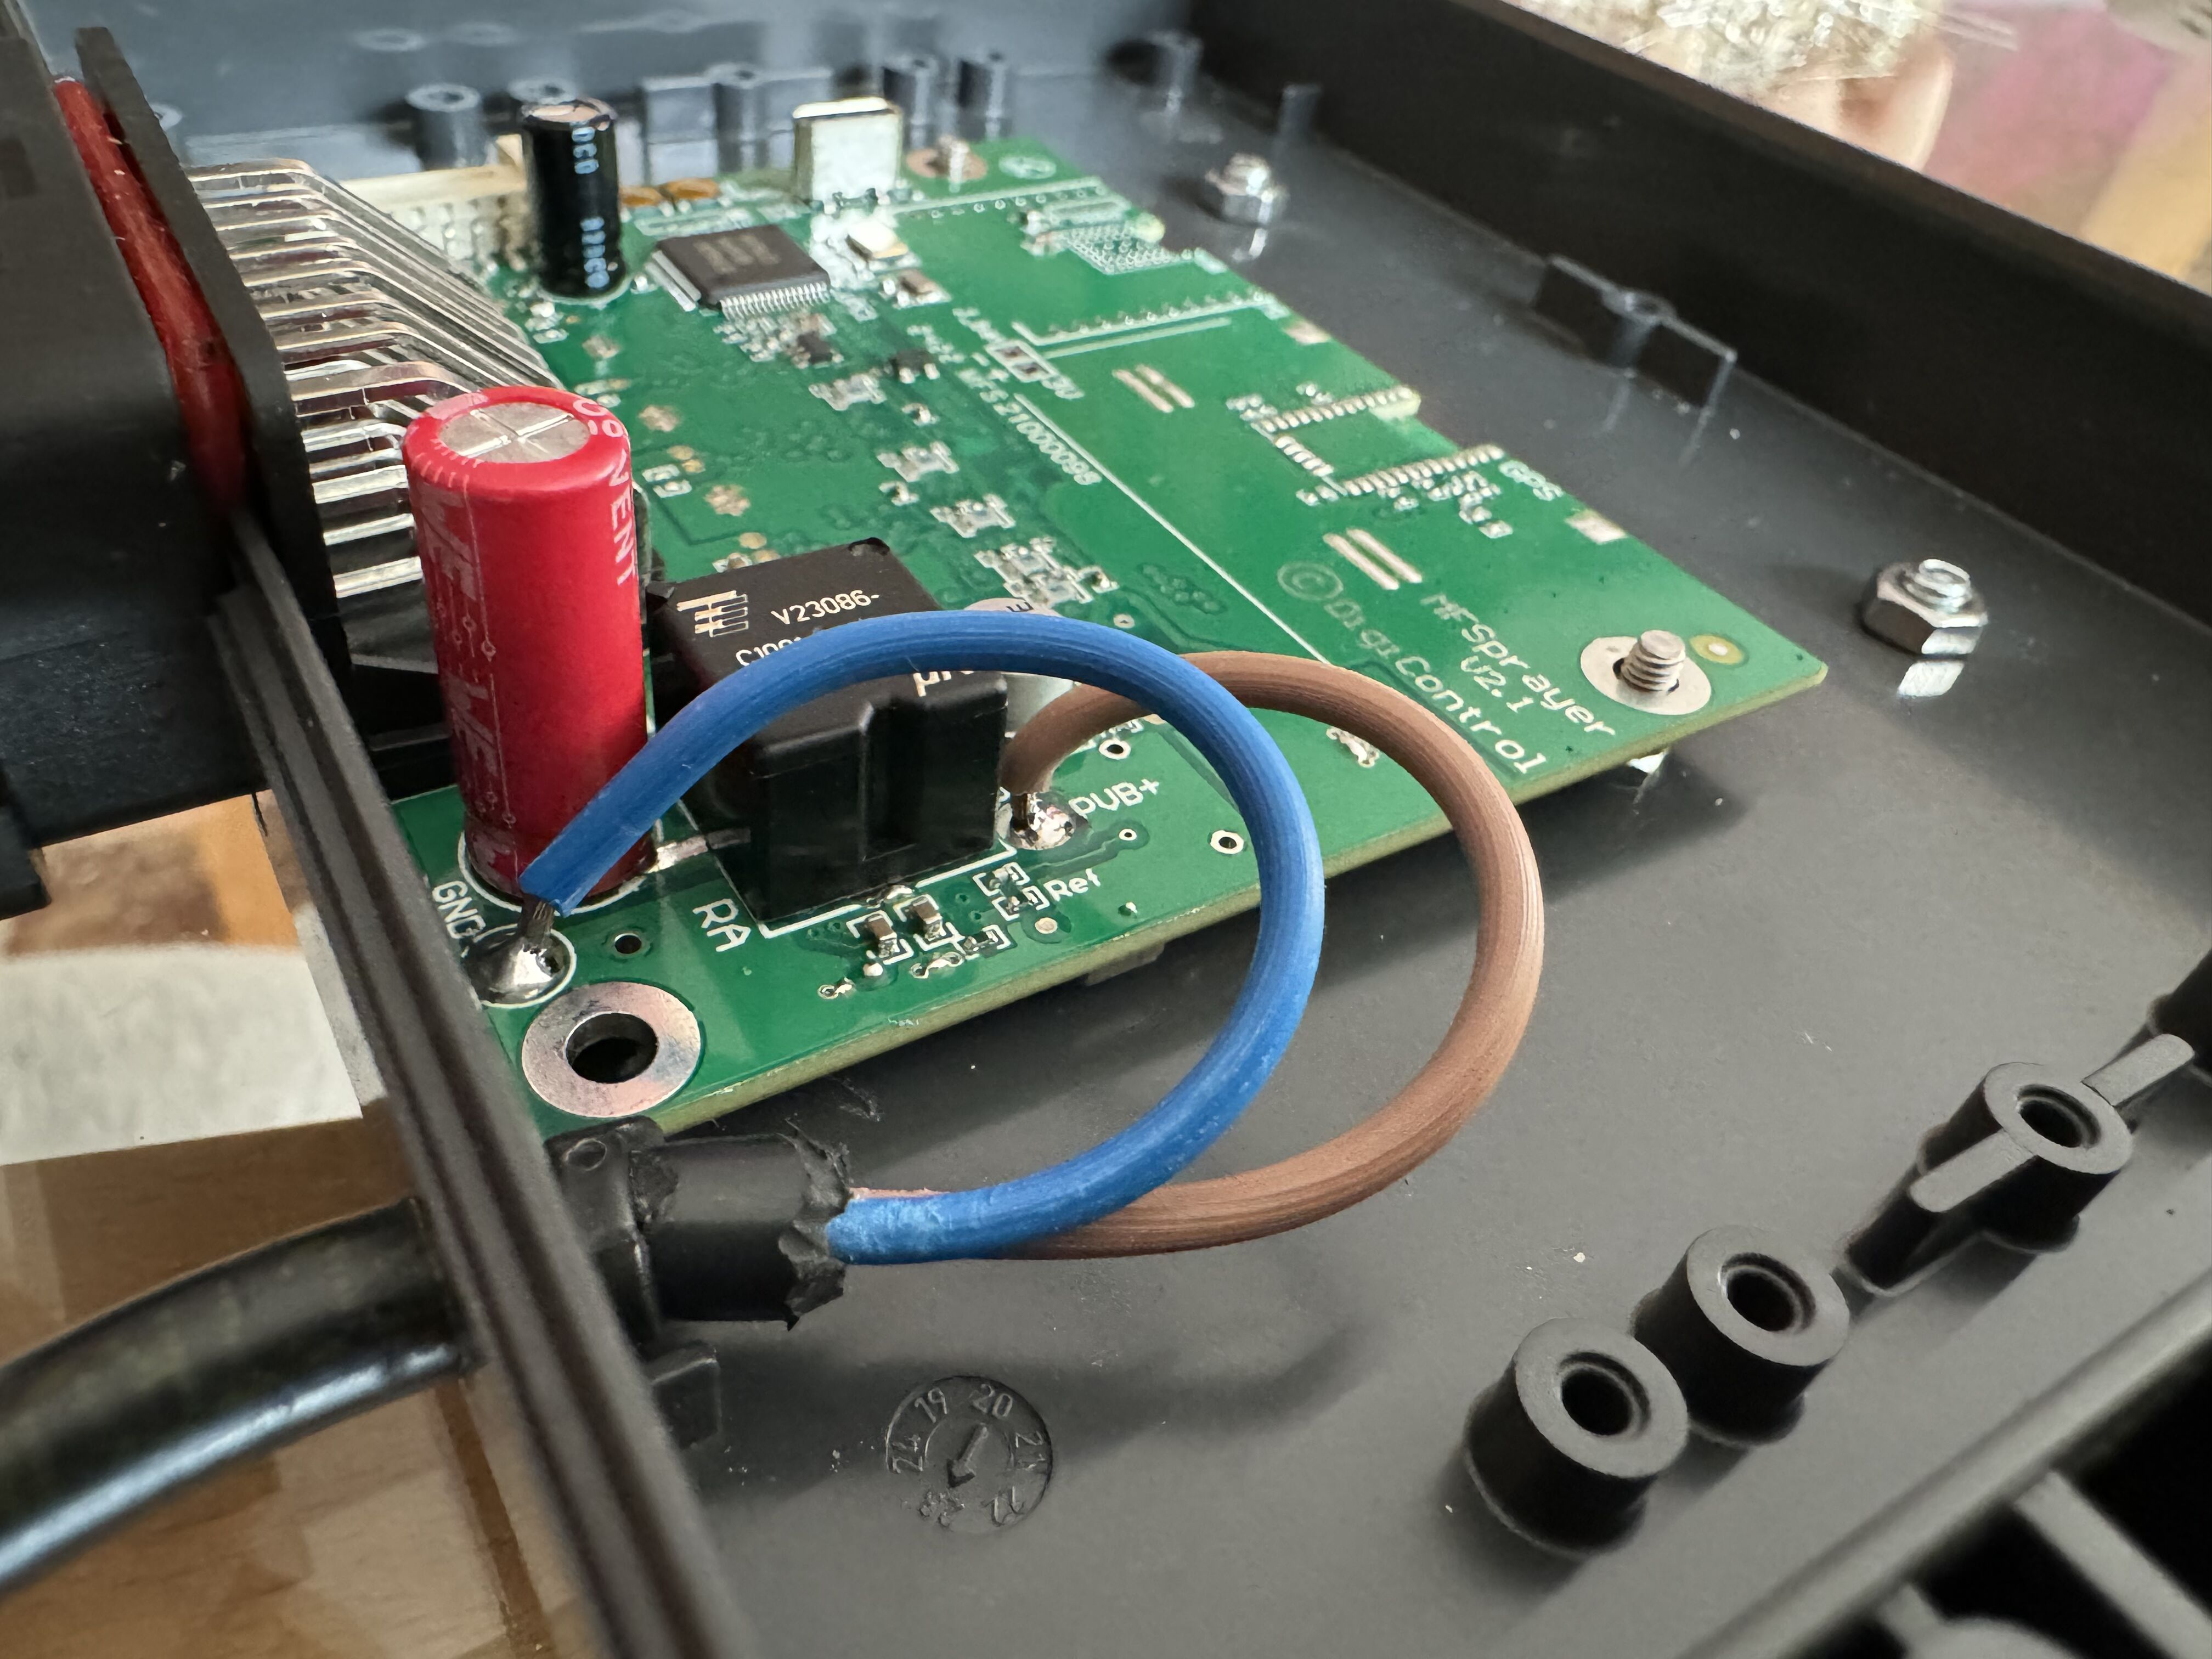
\includegraphics[width=0.55\textwidth]{mfsprayer.jpg}
    \caption{MFSprayer montada en una caja. El código que desarrollamos
    probablemente acabe ampliándose y ejecutándose sobre esta plataforma.}
\end{figure}

\section{Librería Histórico de Registros}

\begin{figure}[h]
    \centering
    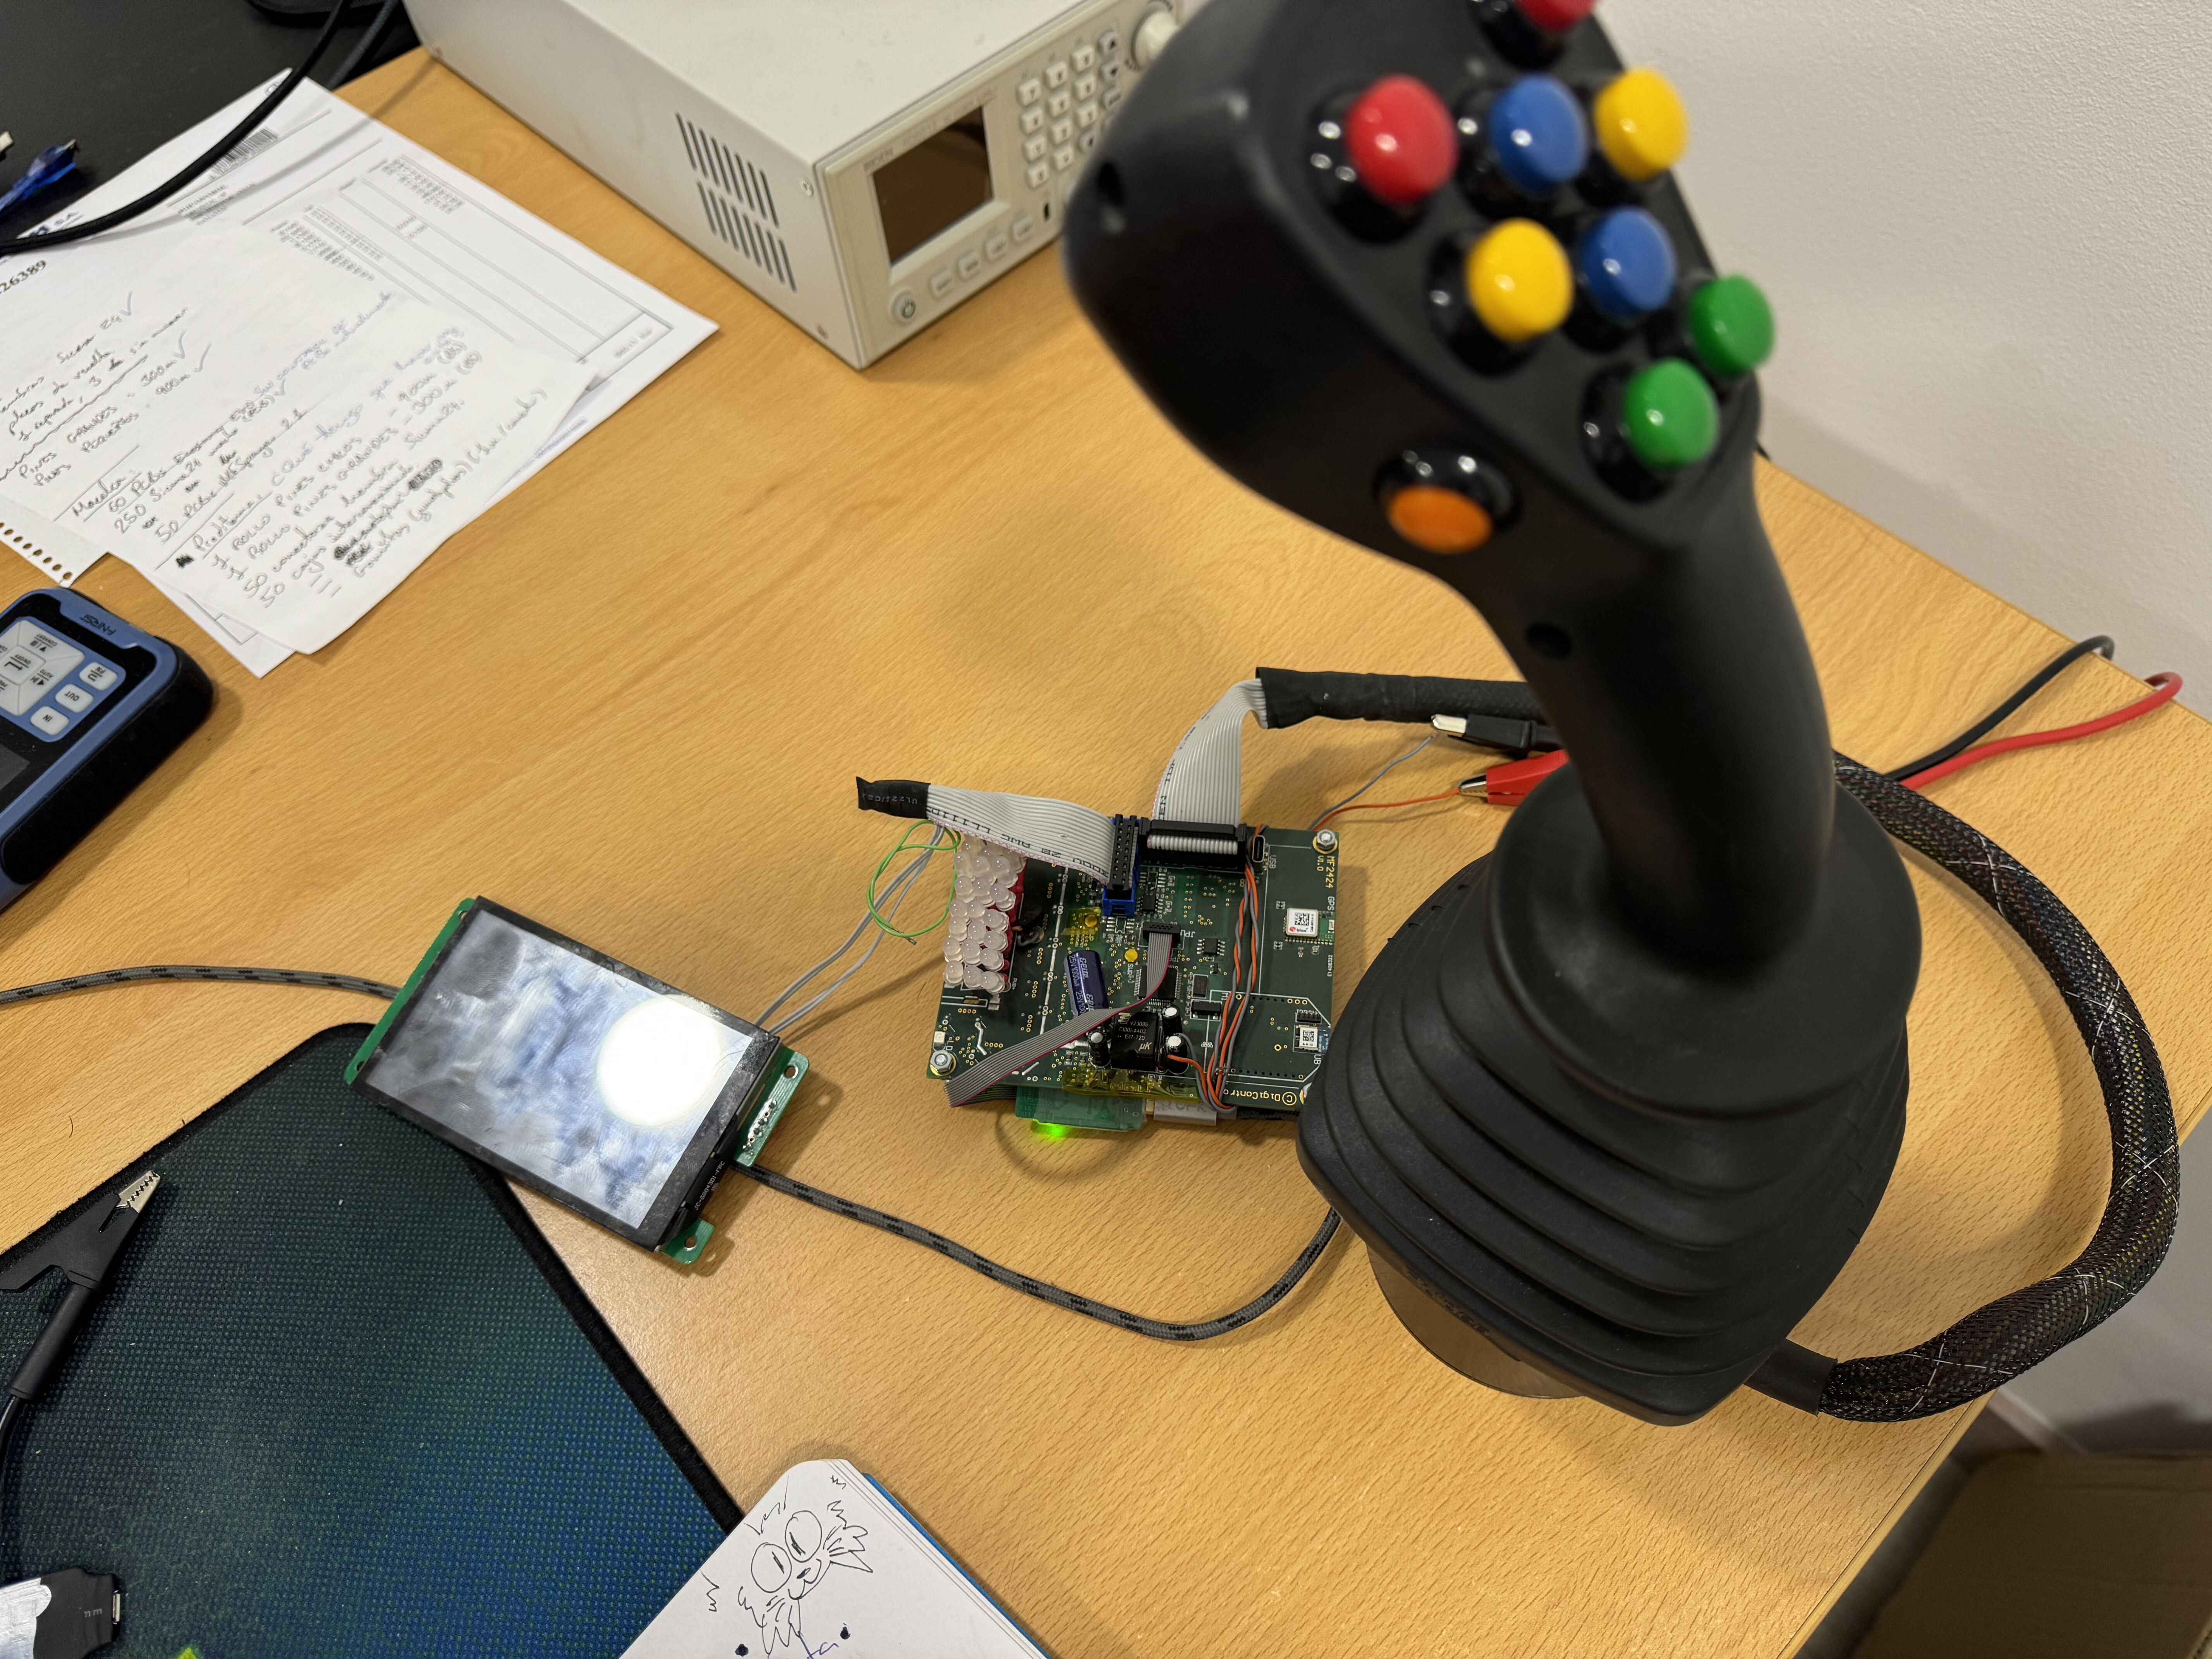
\includegraphics[width=0.55\textwidth]{mf2424-joystick-pantalla.jpg}
    \caption{MF2424v1.0 con Joystick y HMI. Ya que a la hora de desarrollar
    no teníamos todavía un prototipo que montar en un tractor utilizamos
    una plataforma muy parecida en la que probamos mediante pruebas manuales
    que el código de pegamento funciona bien. La MF2424v1.0 no dispone del
    MB85RS4MT, sin embargo, gracias a la inversión de dependencias podemos
    ejecutar el código sobre otro integrado de memoria persistente de menor
    capacidad.}
\end{figure}

Como primer paso y pilar fundamental definimos la interfaz del
módulo. De esta forma tenemos claro desde el principio el propósito
y el ámbito de la librería, tanto en el desarrollo como en el momento
de utilizar la librería en un proyecto.

Decidimos que va a ser responsabilidad de la librería:
\begin{itemize}[noitemsep,nolistsep]
    \item \textbf{Escribir y recuperar de memoria}. Nos da igual
          la memoria subyacente, pero optimizamos para acceso a una
          memoria direccionable a nivel de byte.
    \item \textbf{Extraer información a partir de eventos} que define, y que
          recibe del exterior.
    \item \textbf{Decidir cuándo crear} un registro, \textbf{cuándo trabajar} sobre
          uno existente, etc.
\end{itemize}

Dividimos en una estructura de datos para acceder y recuperar registros de memoria
y en reglas acerca de cómo procesar la información de los eventos que recibimos,
y seguimos en cada submódulo el ciclo \textit{``creamos un nuevo test, hacemos pasar
al test, hacemos refactor del código.''} \cite{TDD}

Definimos en forma de tests el comportamiento de la librería e implementamos
seguidamente siguiendo el mismo ciclo.

\section{Librería MB85RS4MT}

\begin{figure}[h]
    \centering
    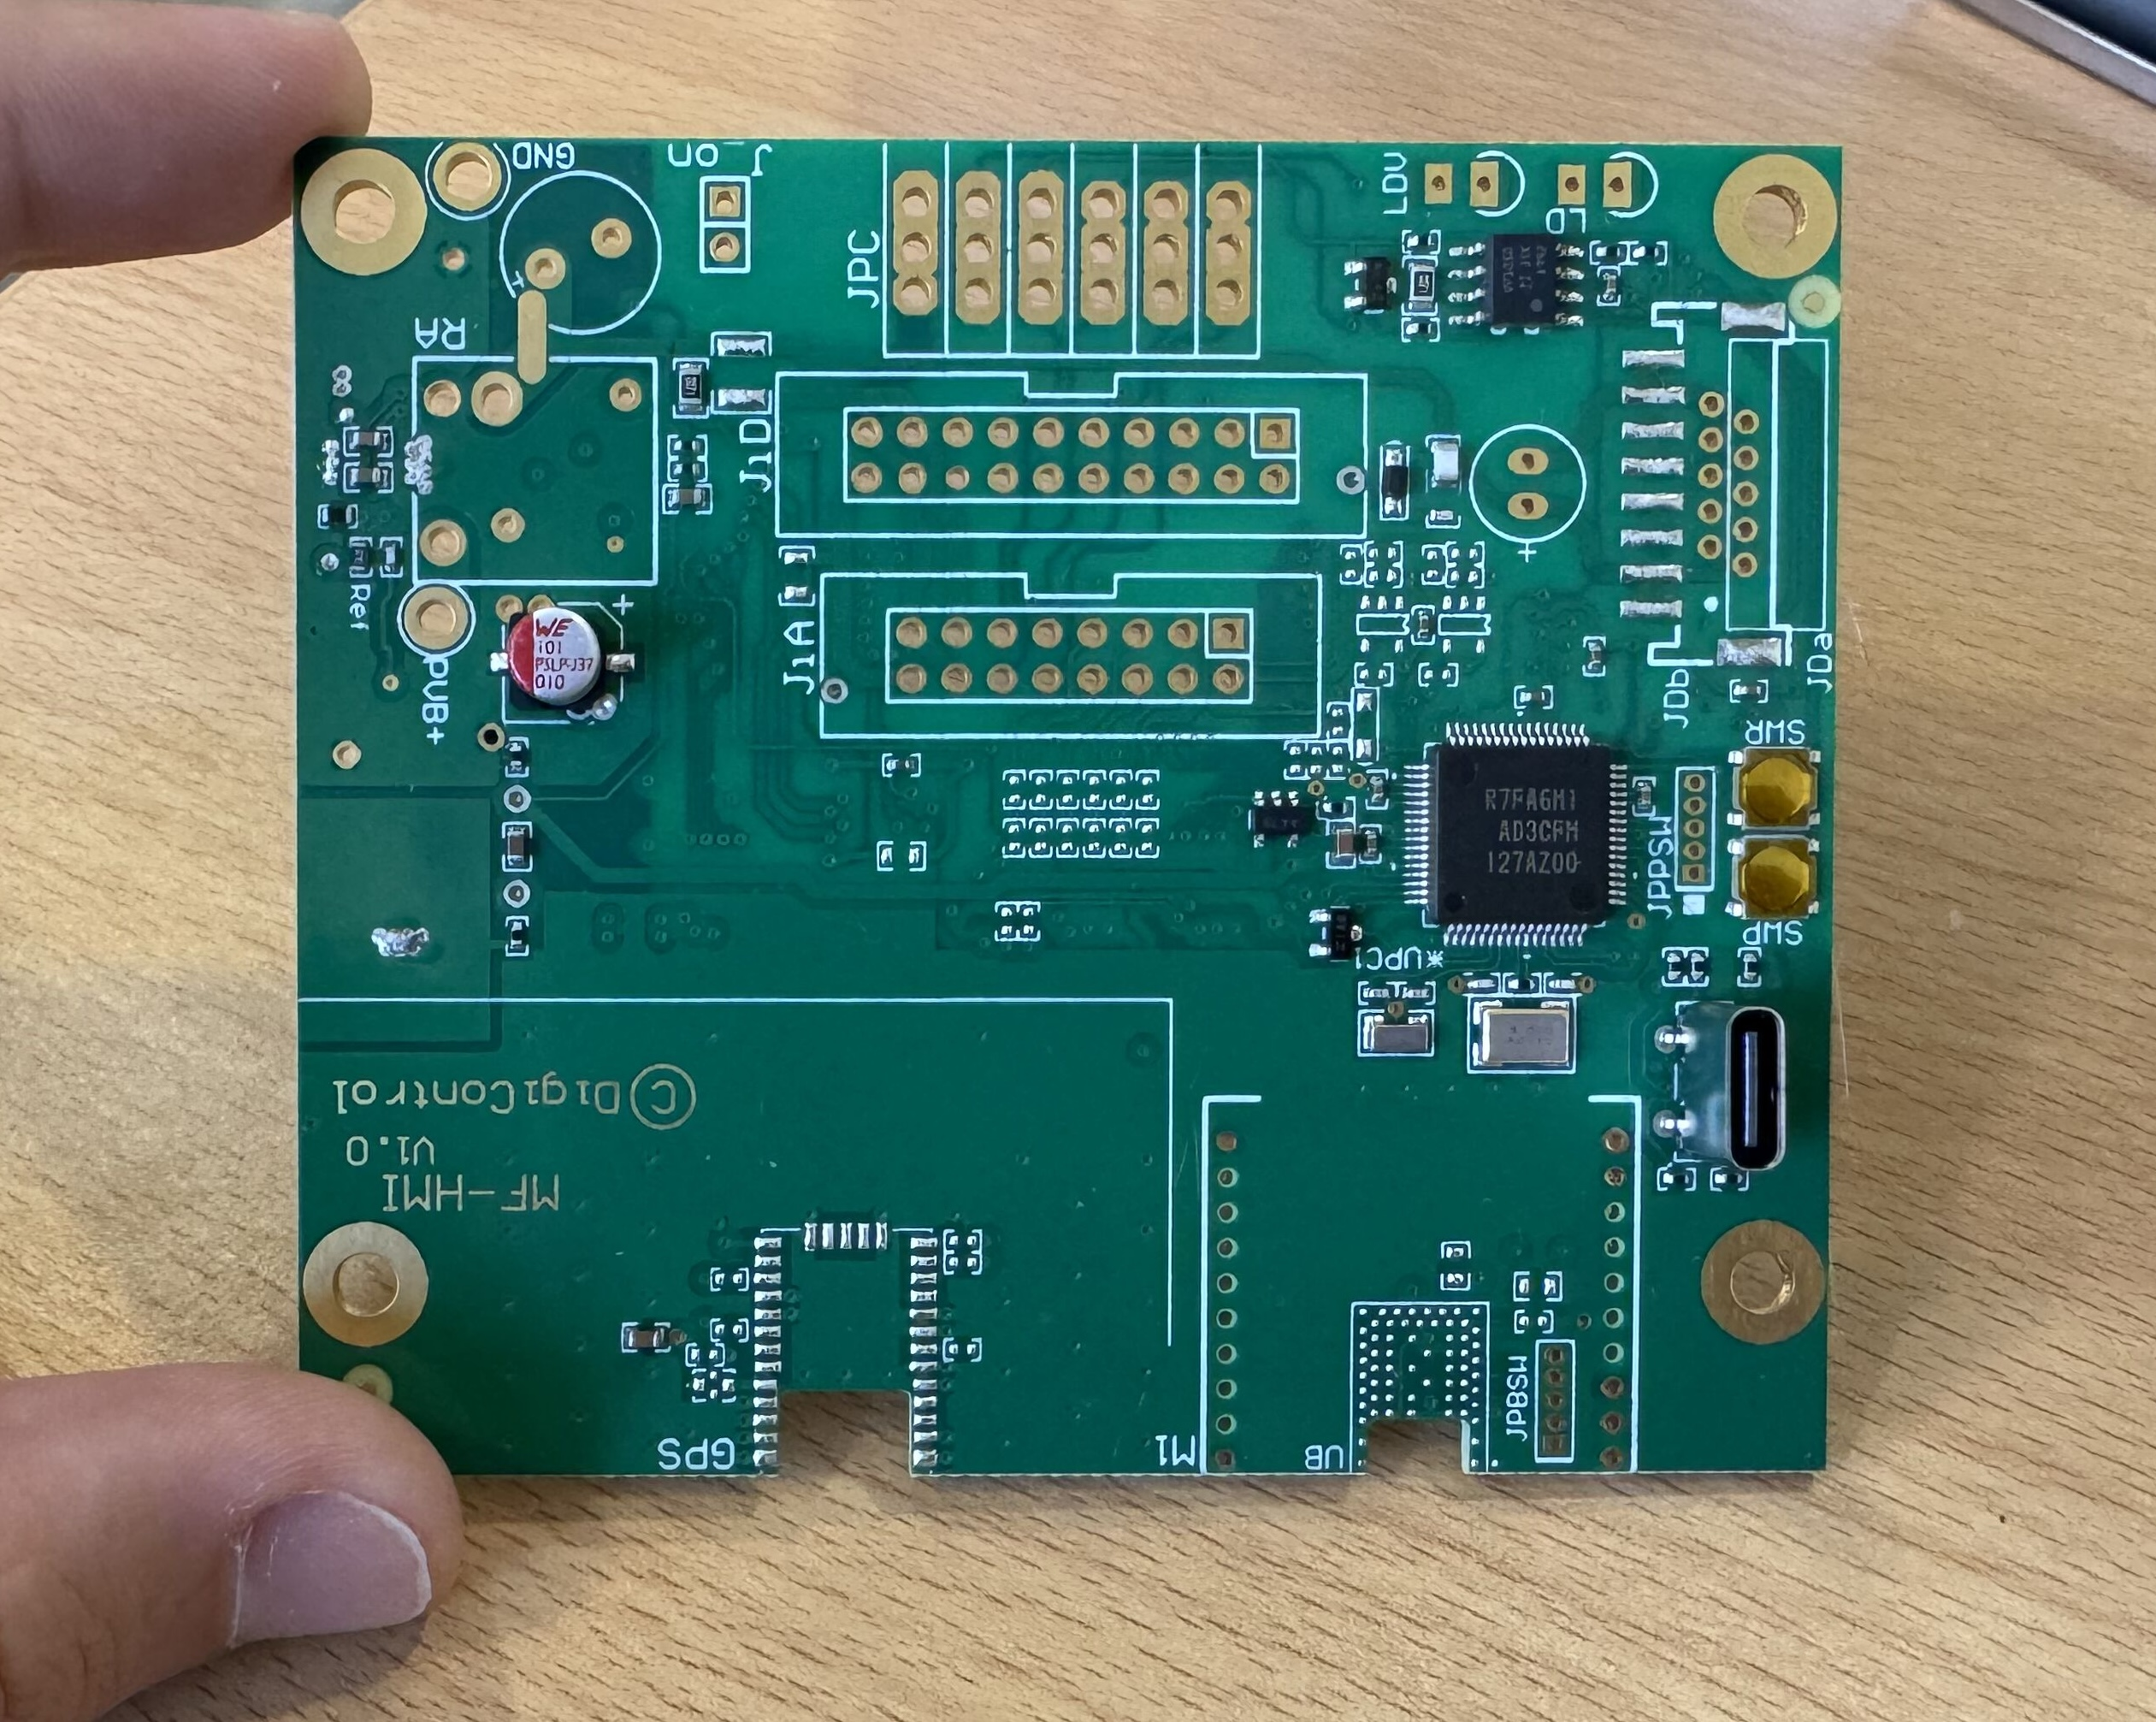
\includegraphics[width=0.55\textwidth]{mfhmi.jpg}
    \caption{MFHMI a falta de soldarle algunos componentes de la fuente de alimentación.
    Ya que todavía no disponíamos de la tarjeta objetivo en la que correrá
    finalmente nuestro programa desarrollamos el driver en una MFHMI que disponía
    del integrado MB85RS4MT.}
\end{figure}

Leemos \textbf{detenidamente} datasheet que ofrece Fujitsu \cite{Fujitsu:MB85RS4MT}.
Vamos implementando, un poco según prueba y error, test a test, el driver.
A partir del cálculo teórico de la hoja de datos técnicos no vemos la
necesidad de hacer el código asíncrono al ser aceptables los tiempos de acceso para
nuestras aplicaciones.
Vamos mejorando mientras la claridad del código. Invertimos sus dependencias. 

Integramos la librería en el BSP que tenemos desarrollado para la plataforma objetivo,
que abstraemos mediante una interfaz que únicamente permite leer y escribir un
número determinado de bytes de forma síncrona.

Hacemos mediciones empíricas del tiempo que tarda en escribir y leer. De media escribió
toda la memoria en 1.53s con el bus SPI trabajando a 16MHz.

\vspace*{\fill}

\pagebreak

\section{Documentación para el cliente}

\subsection{Comunicación acerca del estado del desarrollo del proyecto} \label{sec:plan_de_desarrollo}

Según estimamos o según se nos solicita comunicamos con el cliente el
estado del proyecto mediante el documento ``Plan de Desarrollo''.
En este caso no ha sido de mucha utilidad, porque el ámbito del proyecto
ha sido limitado y porque el desarrollo ha sido muy lineal. Normalmente
este documento se va viendo modificado según las necesidades del cliente,
más cuando el proyecto está en continuo desarrollo.

\begin{figure}[!h]
    \centering
    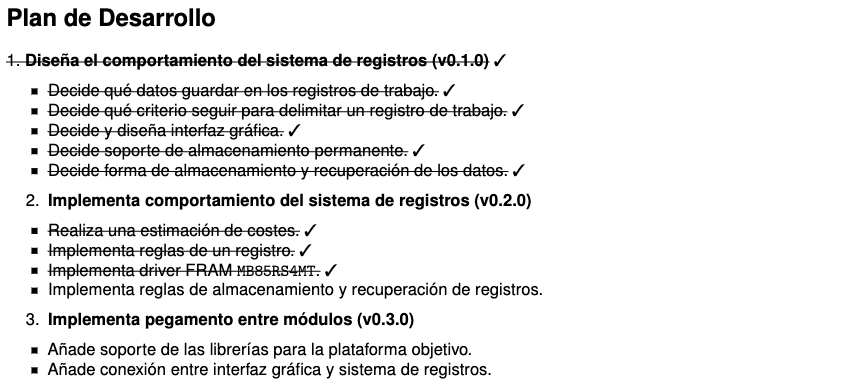
\includegraphics[width=0.9\textwidth]{plan-de-desarrollo.png}
    \caption{\textit{Captura de pantalla del documento ``Plan de Desarrollo''.
    Tachamos las tareas que hemos completado y definimos cuáles serán los
    siguientes pasos que probablemente daremos.}}
\end{figure}

\subsection{Cambios en la última versión}

Cada vez que liberamos una versión incluimos en el comprimido un documento
PDF exponiendo qué ha cambiado con respecto a la última versión. Nos
apoyamos en el historial de \texttt{git} para redactarlo.

\begin{figure}[!h]
    \centering
    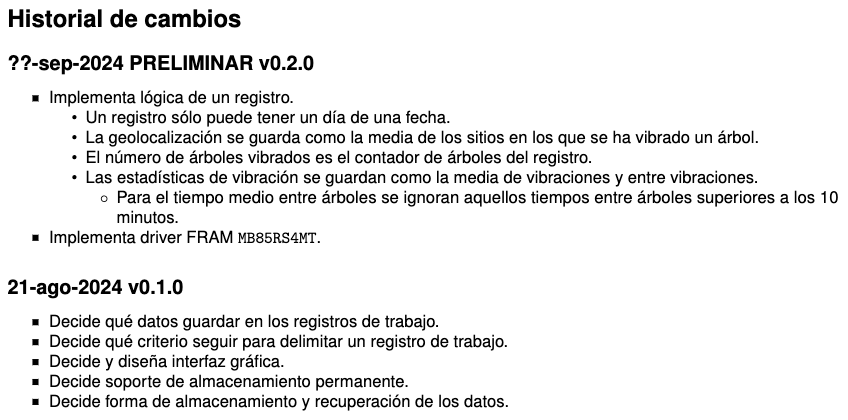
\includegraphics[width=0.9\textwidth]{historial-de-cambios.png}
    \caption{\textit{Captura de pantalla del documento ``Historial de cambios''.
            Explicamos qué cambios han ocurrido en los productos a entregar
            desde la última versión.}}
\end{figure}
